\section{The Product and Quotient Rules}
\label{sec:prod-quot}


The derivative of a sum is the sum of the derivatives, but can we say the same about the derivative of a product or the derivative of a quotient?

\begin{example} Consider $f(x) = x\cdot x$. We know that $f'(x) = 2x$ and $\frac{d}{dx}x = 1$, so clearly, the derivative of a product is not the product of the derivatives. $2x \ne 1\cdot 1$.
\end{example}

\begin{example}
  \label{ex:2-8-1}
Find the derivative of $h(x)=(4x^3-11)(x+3)$.

\begin{solution} We could simply multiply it out to find its derivative.
\begin{align*}
		h(x) &= \left(4x^3-11\right)(x+3)\\
		 &= 4x^4-11x+12x^3-33\\
		h'(x) &= 16x^3-11+36x^2
	\end{align*}
\end{solution}\end{example}
For more complicated examples, this would be unwieldy.

\subsection{The Product Rule}

To motivate the {\bf Product Rule} for derivatives, consider an example of {\bf dollar cost averaging}. Consider units carefully, since that will help us understand the Product Rule.

\begin{example} Suppose you buy a share of a stock each month. When you started investing, at month 0, it was \$100 per share and the price went up at a constant rate of \$1 per month. After one year, at what rate was the value of your investment increasing?

\begin{solution} Let $n(m)$ be the number of shares of stock you own after $m$ months and let $s(m)$ be the value of a share of stock after $m$ months. The total value of your investment after $m$ months is $v(m) = n(m)\cdot s(m)$. We want to know $v'(m)$ and $v'(12)$. After 12 months, $n(12) = 12$ shares and $n'(12) = 1$ share per month. $v(12) = \$120$ per share and $v'(12) = \$1$ per share per month. The units on $v'(m)$ is dollars per month. The increase in the value of your investment comes from the increase in the price of each share that you currently have plus the monthly investment of one share. This is a sum of two components.
\begin{align*}
v'(12) \,\frac{\text{dollars}}{\text{month}} &=  \text{ increase from share value } + \text{ increase from monthly investment } \\
    &= \left( n'(12) \,\frac{\text{shares}}{\text{month}} \right) \left( v(12)\,\frac{\text{dollars}}{\text{share}} \right) + \left(  n(12)\, \text{ shares }\right)\left( v'(12)\, \frac{\text{dollars}}{\text{share}\cdot \text{month}} \right) \\
&= \left( 1 \,\frac{\text{share}}{\text{month}} \right) \left( 120 \,\frac{\text{dollars}}{\text{share}} \right) + \left(  12 \,\text{ shares }\right)\left( 1\, \frac{\text{dollar}}{\text{share}\cdot \text{month}} \right) \\
&= 120 \,\frac{\text{dollars}}{\text{month}}+ 12 \,\frac{\text{dollars}}{\text{month}}\\
&= 132 \,\frac{\text{dollars}}{\text{month}}
\end{align*}
After 1 year, the value of the investment is growing at a rate of \$132 per month. 
\end{solution}\end{example}

In general, we see that $v'(m) = n'(m)v(m) + n(m)v'(m)$; the units in both terms on the right are ``dollars per month'' after we cancel the unit ``shares." Without writing out a formal proof, the intuition from this example leads us to generalize this example. 

\begin{theorem}[Product Rule\index{Product Rule}]
If $f(x)$ and $g(x)$ are differentiable, then
$\dfrac{d}{dx}\left( f(x)\cdot g(x) \right)=f'(x)\cdot g(x)+f(x)\cdot g'(x) \enspace .$
\end{theorem}

The derivative of the first factor times the second left alone, plus the first left alone times the derivative of the second.

The Product Rule can extend to a product of several functions; the pattern continues -- take the derivative of each factor in turn, multiplied by all the other factors left alone, and add them up:
$$\dfrac{d}{dx} f(x)\cdot g(x)\cdot h(x) = f'(x)\cdot g(x)\cdot h(x)+f(x)\cdot g'(x)\cdot h(x)+f(x)\cdot g(x)\cdot h'(x) \enspace .$$


\begin{example}
Use the Product Rule to find the derivative of $h(x)=(4x^3-11)(x+3)$.

\begin{solution} This is the same function we found the derivative of in Example \ref{ex:2-8-1} , but let's use the Product Rule and check to see if we get the same answer. For this first example, we will provide a lot more detail and steps than one usually actually shows when working a problem like this.

Notice we can think of $h(x)$ as the product of two functions $f(x)=4x^3-11$ and $g(x)=x+3$. Finding the derivative of each of these,
$f'(x)=12x^2$ and $g'(x)=1$.
Using the Product Rule, we have: 
\begin{align*}
		h'(x) &= (f')(g)+(f)(g') \\
		 &= \left(12x^2\right)(x+3)+\left(4x^3-11\right)(1)
	\end{align*}
To check if this is equivalent to the answer we found in Example \ref{ex:2-8-1}  we could simplify:
\begin{align*}
		h'(x) &= \left(12x^2\right)(x+3)+\left(4x^3-11\right)(1) \\
		 &= 12x^3+36x^2+4x^3-11 \\
		 &= 16x^3+36x^2-11
	\end{align*}
From this, we can see the answers are equivalent.
\end{solution}\end{example}



\begin{example}
Find the derivative of $ F(t)=e^t\ln(t) $.

\begin{solution} This is a product, so we need to use the Product Rule. 
$$F'(t)=\left(e^t\right)\left(\ln(t)\right)+\left(e^t\right)\left(\dfrac{1}{t}\right)=e^t\ln(t)+\dfrac{e^t}{t}$$
\end{solution}\end{example}

Notice that this was one we could not have done by multiplying out.


\subsection{The Quotient Rule}
\begin{theorem}[Quotient Rule\index{Quotient Rule}]
$$\dfrac{d}{dx}\dfrac{f(x)}{g(x)} = \dfrac{f'(x)\cdot g(x)-f(x)\cdot g'(x)}{g^2(x)}$$
\end{theorem}
An easy way to remember this is with a chant.\\

``Low dee high

minus high dee low

over low squared

it's the way to go.''

The numerator of the result resembles the Product Rule, but there is a minus instead of a plus; the minus sign goes with the $g'(x)$. The denominator is simply the square of the original denominator -- no derivatives there.

\begin{example}
Find the derivative of $ y=\dfrac{x^4+4^x}{3+16x^3} $.

\begin{solution} This is a quotient, so we need to use the Quotient Rule.
$$y'=\dfrac{\left(4x^3+\ln(4)\cdot 4^x \right)\left(3+16x^3 \right)-\left(x^4+4^x \right)\left(48x^2 \right)}{\left(3+16x^3 \right)^2}$$
\end{solution}\end{example}

Now for goodness' sake don't try to simplify that! Remember that simple depends on what you will do next; in this case, we were asked to find the derivative, and we've done that. I expect you to do any basic simplifications, such as multiplying constants together or doing obvious cancellations or combining of terms, but otherwise please STOP unless there is a reason to simplify further.

\begin{example}
Suppose a large tank contains 8 kg of a chemical dissolved in 50 liters of water. If a tap is opened and water is added to the tank at a rate of 5 liters per minute, at what rate is the concentration of chemical in the tank changing after 4 minutes?

\begin{solution} First we need to set up a model for the concentration of chemical. The concentration would be measured as kg of chemical per liter of water, kg/L. The number of kg of chemical stays constant at 8 kg, but the quantity of water in the tank is increasing at a constant rate of 5 L/min. The total volume of water in the tank after t minutes is $50+5t$, so the concentration after $t$ minutes is
$$c(t)=\dfrac{8}{50+5t} \enspace .$$
To find the rate at which the concentration is changing, we need the derivative:
\begin{align*}
			c'(t) &= \dfrac{\dfrac{d}{dt}(8)\cdot(50+5t)-(8)\cdot\dfrac{d}{dt}(50+5t)}{(50+5t)^2} \\
			 &= \dfrac{(0)\cdot(50+5t)-(8)(5)}{(50+5t)^2} \\
			 &= -\dfrac{40}{(50+5t)^2} \enspace .
		\end{align*}
At $t=4$ minutes, we have 
$$ c'(4)=-\dfrac{40}{(50+5(4))^2}\approx -0.00816 \enspace .$$
Note that the units here are kg per liter, per minute, or $ \dfrac{\text{kg/L}}{\text{min}} $. In other words, this tells us that after 4 minutes, the concentration of chemical is decreasing at a rate of 0.00816 kg/L per minute.
\end{solution}\end{example}

\subsection{More Graphical Interpretations of the Basic Business Math Terms}
Returning to our discussion of business and economics topics, in addition to total cost\index{Cost} and marginal cost\index{Marginal cost}, we often also want to talk about average cost\index{Average cost}\index{Cost!average} or average revenue\index{Average revenue}\index{Revenue!average}.

Recall from Section \ref{sec:functions} (Definition \ref{def:avgcost} that the average cost for $q$ items is the total cost divided by $q$, or $A(q)=\dfrac{C(q)}{q}$. You can also talk about the average fixed cost, $\dfrac{FC(q)}{q}$, or the average variable cost, $\dfrac{VC(q)}{q}$.

Also recall that the Average Revenue (AR) for $q$ items is the total revenue divided by $q$, or $AR(q)=\dfrac{R(q)}{q}$. But $\dfrac{R(q)}{q} = \dfrac{q \cdot D(q)}{q}= D(q)$, so $AR(q)=D(q)$, which just the price since $p=D(q)$.

We already know that we can find average rates of change by finding slopes of secant lines. AC, AR, MC, and MR are all rates of change, and we can find them with slopes too.

$AC(q)$ is the slope of a diagonal line, from $(0, 0)$ to $(q,C(q))$.

$AR(q)$ is the slope of the line from $(0, 0)$ to $(q,R(q))$, which is the also equal to the price at $(q,R(q))$ by the calulations in the previous paragraph.

\begin{figure}[!ht]
  \centering
    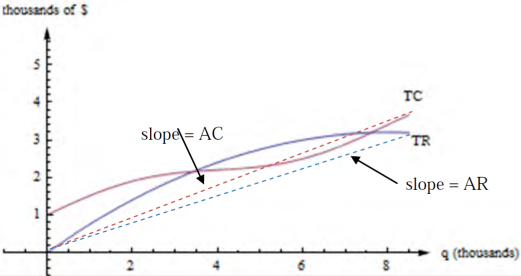
\includegraphics[width=0.4\textwidth]{img/chap2/image113.png}
    %\caption{$y=g(x)$}
    %\label{fig:2-2-gx}
\end{figure}

And just as we found marginal Total Cost, we can also find marginal Average Cost.

\begin{example}
The cost, in thousands of dollars, for producing $x$ thousand cell phone cases is given by $C(x)=22+x-0.004x^2$. Find
    \begin{enumerate}[label=(\alph*)]
    \item the Fixed Costs,

    \begin{solution}
    The fixed costs are the costs when no items are produced: $C(0)=22$ thousand dollars.
    \end{solution}
    \item the Average Cost when 5 thousand, 10 thousand, or 20 thousand cases are produced,

    \begin{solution}
    The average cost function is total cost divided by number of items, so
$$AC(x)=\dfrac{C(x)}{x}=\dfrac{22+x-0.004x^2}{x}. $$
Note the units are thousands of dollars per thousands of items, which simplifies to just dollars per item.

At a production of 5 thousand items: $ AC(5)=\dfrac{22+5-0.004(5)^2}{5}=5.38 $ dollars per item.

At a production of 10 thousand items: $ AC(10)=\dfrac{22+5-0.004(10)^2}{10}=3.16 $ dollars per item.

At a production of 20 thousand items: $ AC(20)=\dfrac{22+5-0.004(20)^2}{20}=2.02 $ dollars per item.

Notice that while the total cost increases with production, the average cost per item decreases, because the initial fixed costs are being distributed across more items.
    \end{solution}
    \item the Marginal Average Cost when 5 thousand cases are produced.

    \begin{solution} 
    For the marginal average cost, we need to find the derivative of the average cost function. We can either calculate this using the Quotient Rule, or we could use algebra to simplify the equation first (this is the easier option -- remember, simplifying before differentiating is almost always easier):
    \begin{align*}
					AC(x) &= \dfrac{22+x-0.004x^2}{x} \\
					 &= \dfrac{22}{x}+\dfrac{x}{x}-\dfrac{0.004x^2}{x} \\
					 &= \dfrac{22}{x}+1-0.004x \\
					 &= 22x^{-1}+1-0.004x
\end{align*}
(Note: We haven't differentiated yet, only simplified.)

Taking the derivative,
$$ AC'(x)=-22x^{-2}-0.004=-\dfrac{22}{x^2}-0.004 \enspace .$$
When 5 thousand items are produced,
$$ AC'(5)=-\dfrac{22}{5^2}-0.004=-0.884 \enspace .$$
Since the units on $AC(x)$ are dollars per item, and the units on $x$ are thousands of items, the units on $AC'(x)$ are dollars per item per thousands of items. This tells us that when 5 thousand items are produced, the average cost per item is decreasing at a rate of \$0.884 per additional thousand items produced.
    \end{solution}
    \end{enumerate}
\end{example}
